% !TEX root = ../main.tex
% Einleitung

Das Bedürfnis, Informationen anschaulich darzustellen, ist ein Phänomen, das die Kulturgeschichte des Menschen seit der Frühzeit begleitet.
Eine der ältesten visuellen Metaphern ist der Baum.
So beschreibt Lima \cite[S. 9]{lima2014book} im Vorwort seines Buches \emph{The book of trees: Visualizing branches of knowledge} den Baum als einen \" visuellen Archetypen\" . \footnote{ \"(...)the tree as one of the most popular, captivating, and widespread visual archetypes." \cite[S. 9]{lima2014book}}
Der Baum kann als Repräsentation auf unterschiedlichste Art und Weise grafisch übersetzt werden.
Das Spektrum reicht von nahezu realistischen Darstellungen bis hin zu abstrakten Formen, reduziert auf Knoten und Kanten.
Als visuelle Metapher zur Darstellung von Informationen kommen Baumdiagramme in vielen Bereichen zum Einsatz; z.\,B. zur Darstellung von Erbfolgen, beim sogenannten Stammbaum, oder um Rangordnungen im Tierreich abzubilden. \cite{lima2014book}

Im Besonderen macht sich diese Darstellungsform die Hierarchie und geordnete Struktur eines Baumes zu Nutzen.
So lässt sich der Baum als eine visuelle Repräsentation verstehen, mit deren Hilfe sich komplexe Beziehungen zwischen einzelnen Entitäten übersichtlich darstellen lassen \cite[S. 43]{lima2014book}.

Diese Arbeit beschäftigt sich mit der visuellen Metapher des Baumes als eine Möglichkeit zur Darstellung der Kategorienstruktur der Wikipedia und versucht die Ähnlichkeiten zwischen Artikeln auf Paragrafenebene innerhalb eines Themenbereichs visuell kenntlich zu machen.
Die Arbeit zielt darauf ab, die inhaltlichen Zusammenhänge der Themengebiete der Enzyklopädie Wikipedia grafisch darzustellen.
Dem Nutzer wird damit die Möglichkeit gegeben, die Darstellung flexibel, interaktiv und in Echtzeit nach seinen Intentionen bzw. Parametern zu verändern.

\section{Motivation}\label{subchap:motivation}
Die Grundlage der vorliegenden Arbeit bilden die Erkenntnisse des Projekts \emph{Visual Text Analytics}, entstanden an der Fakultät Medien der Bauhaus-Universität Weimar am Lehrstuhl Virtuelle Realität.
Dieses Projekt setzte sich bereits zum Ziel, die Ähnlichkeiten zwischen den Artikeln der Wikipedia zu visualisieren.
In der Darstellung werden die Artikel als Knoten dargestellt, wohingegen die Kanten eine vorhandene Ähnlichkeit zwischen zwei Artikeln abbilden.

Die Intention des Projekts bestand darin, die inhaltlichen Überschneidungen einer möglichst großen Anzahl von Wikipedia-Artikeln sowie ihrer Ähnlichkeitswerte, wie in Abbildung \ref{fig:vta-cover} zu sehen, darzustellen.
Im Voraus wird ein Schwellwert für die Ähnlichkeitswerte zwischen den Artikeln festgelegt, welcher maßgeblich die Anordnung der Artikel in der Visualisierung bestimmt.
Ähnlichkeitswerte unter dem Schwellwert werden nicht mit einbezogen und folglich nicht dargestellt. 
Die auf diese Weise gefilterten, oberhalb des Schwellwerts liegenden Artikel werden dabei in Gruppen von ähnlichen Artikeln, sogenannten Clustern, zusammengefasst.
\footnote{Im Kapitel \ref{subchap:simmatrix} wird im Detail auf die Berechnung der Ähnlichkeiten eingegangen.}

Zusätzlich wird eine zweite, die Darstellung der Artikel unterstützende, Visualisierung der zugehörigen Wikipedia-Kategorien als Graph erarbeitet.
In dieser Darstellung werden Kategorien auch als Knoten abgebildet, wohingegen Kanten eine Verknüpfung von zwei Kategorien bedeuten.
Der die Wikipedia-Kategorien abbildende Graph soll eine verständliche Zusammenfassung auf einer höheren Abstraktionsebene für die Menge der erfassten Wikipedia-Artikel ermöglichen, wie in der Abbildung \ref{subchap:simmatrix} verdeutlicht.


%Diese Vorgehensweise erschwert jedoch eine dynamische Darstellung, da die Bestimmung eines Schwellwerts die Anordnung der Knoten und Kanten festlegt, weshalb der Schwellwert für die Dauer des Programms statisch bleibt.
%Es besteht die Möglichkeit den Schwellwert zu ändern, doch dadurch würden die neu gezeichneten Kanten so angeordnet, dass eine Vielzahl an Überlappungen entstünden.

\section{Problemstellung und Zielsetzung}
Die im Laufe des Projekts \emph{Visual Text Analytics} identifizierten Probleme geben den Anstoß für die Entwicklung einer neuen Herangehensweise an die Visualisierung.
Im Folgendem wird auf die für diese Arbeit relevanten Erkenntnisse kurz eingegangen:
Die Visualisierung der Artikelähnlichkeiten in Gruppen von Artikeln, sogenannten Artikelclustern, wird durch einen definierten Schwellwert erzeugt.
Der Schwellwert bestimmt, wie weit die Ähnlichkeitsmatrix traversiert wird.
Die Herabsetzung des Schwellwerts durch den Nutzer führt zu einer steigenden Anzahl an zu traversierenden Artikelähnlichkeiten aus der Ähnlichkeitsmatrix.
Durch den herabgesetzten Schwellwert wird eine größere Anzahl von Artikelähnlichkeiten in Betracht gezogen.
Dies führt zu neu erzeugten Artikelclustern.
Für diese neu entstandenen Artikelcluster muss eine neue Visualisierung gezeichnet werden.
Da die Anzahl der zu betrachtenden Artikelähnlichkeiten gestiegen ist, steigt auch die Dauer der Berechnung der neuen Darstellung.
Die wachsende zeitliche Verzögerung führt dazu, dass die Visualisierung statisch wirkt, wodurch keine unmittelbare Interaktion zustande kommt.

Um die zeitaufwendige Berechnung der Anordnung zu umgehen, können die Artikelähnlichkeiten, die durch den herabgesetzten Schwellwert einbezogen  werden, der bestehenden Visualisierung in Form von Kanten hinzugefügt werden. 
Daraus resultiert jedoch eine massive Überzeichnung der Elemente, was folglich die Nachvollziehbarkeit der in der Visualisierung dargestellten Informationen erschwert.

Daraus lässt sich schließen, dass die Größe der Ähnlichkeitsmatrix Auswirkungen auf die Anordnung, das Verständnis und die Interaktivität der Visualisierung hat.
Aus den genannten Gründen sucht diese Arbeit nach einem Ansatz, die Größe der Ähnlichkeitsmatrix zu beeinflussen:\\
Der Fokus dieser Forschungsarbeit liegt im Gegensatz zur vorherigen Arbeit \emph{Visual Text Analytics} nicht auf den Artikeln, sondern auf den Kategorien der Wikipedia, mit deren Hilfe die Größe der Ähnlichkeitsmatrix reduziert und eine neue Form der visuellen Darstellung geschaffen werden soll.\\
Durch letztere wird ein neuer Zugang geschaffen, welcher die Verbindungen zwischen den Kategorien aufdeckt.
Zudem soll dem Nutzer der Visualisierung ermöglicht werden, nach allen verfügbaren Kategorien der Wikipedia zu suchen und die Verbindungen der Kategorien zueinander dynamisch zu erweitern und zu erforschen.
Diese interaktive Exploration der Visualisierung bildet den Mittelpunkt der vorliegenden Arbeit, welche somit einen Beitrag zum Forschungsbereich der Enzyklopädie Wikipedia leistet.


% auf Basis von Ähnlichkeiten zwischen den verglichenen Artikeln die inhaltlichen Ähnlichkeiten zwischen Kategorien für den Nutzer anzeigt.
% Stattdessen sollen Parameter, wie zugehörige Kategorien oder der Schwellwert, den betrachteten Datensatz filtern
% Des Weiteren setzt sich die Arbeit mit der Entwicklung einer Strategie auseinander, die eine dünn besetzte Matrix in der Größe von 643 GB zugänglich macht.
% Eine Anforderung, die an die Visualisierung gestellt wird, ist, eine Anordnung von Knoten und Kanten zu finden, deren Überlappung möglichst gering ist.
% Durch das massive Überzeichnen der Elementen wurde es erschwert, der Visualisierung Informationen zu entnehmen. 
% Die damit einhergehende eingeschränkte Interaktivität mit den Daten ist eines der grundlegenden Probleme, das im Rahmen des Projekts \emph{Visual Text Analytics} auftrat.
% Die Änderung des Schwellwerts während der Visualisierung, um eine vorhandene Ähnlichkeit in Form von Kanten hinzuzufügen, ist nicht ohne eine Überlappung dieser Kanten möglich.


\begin{figure}
\centering
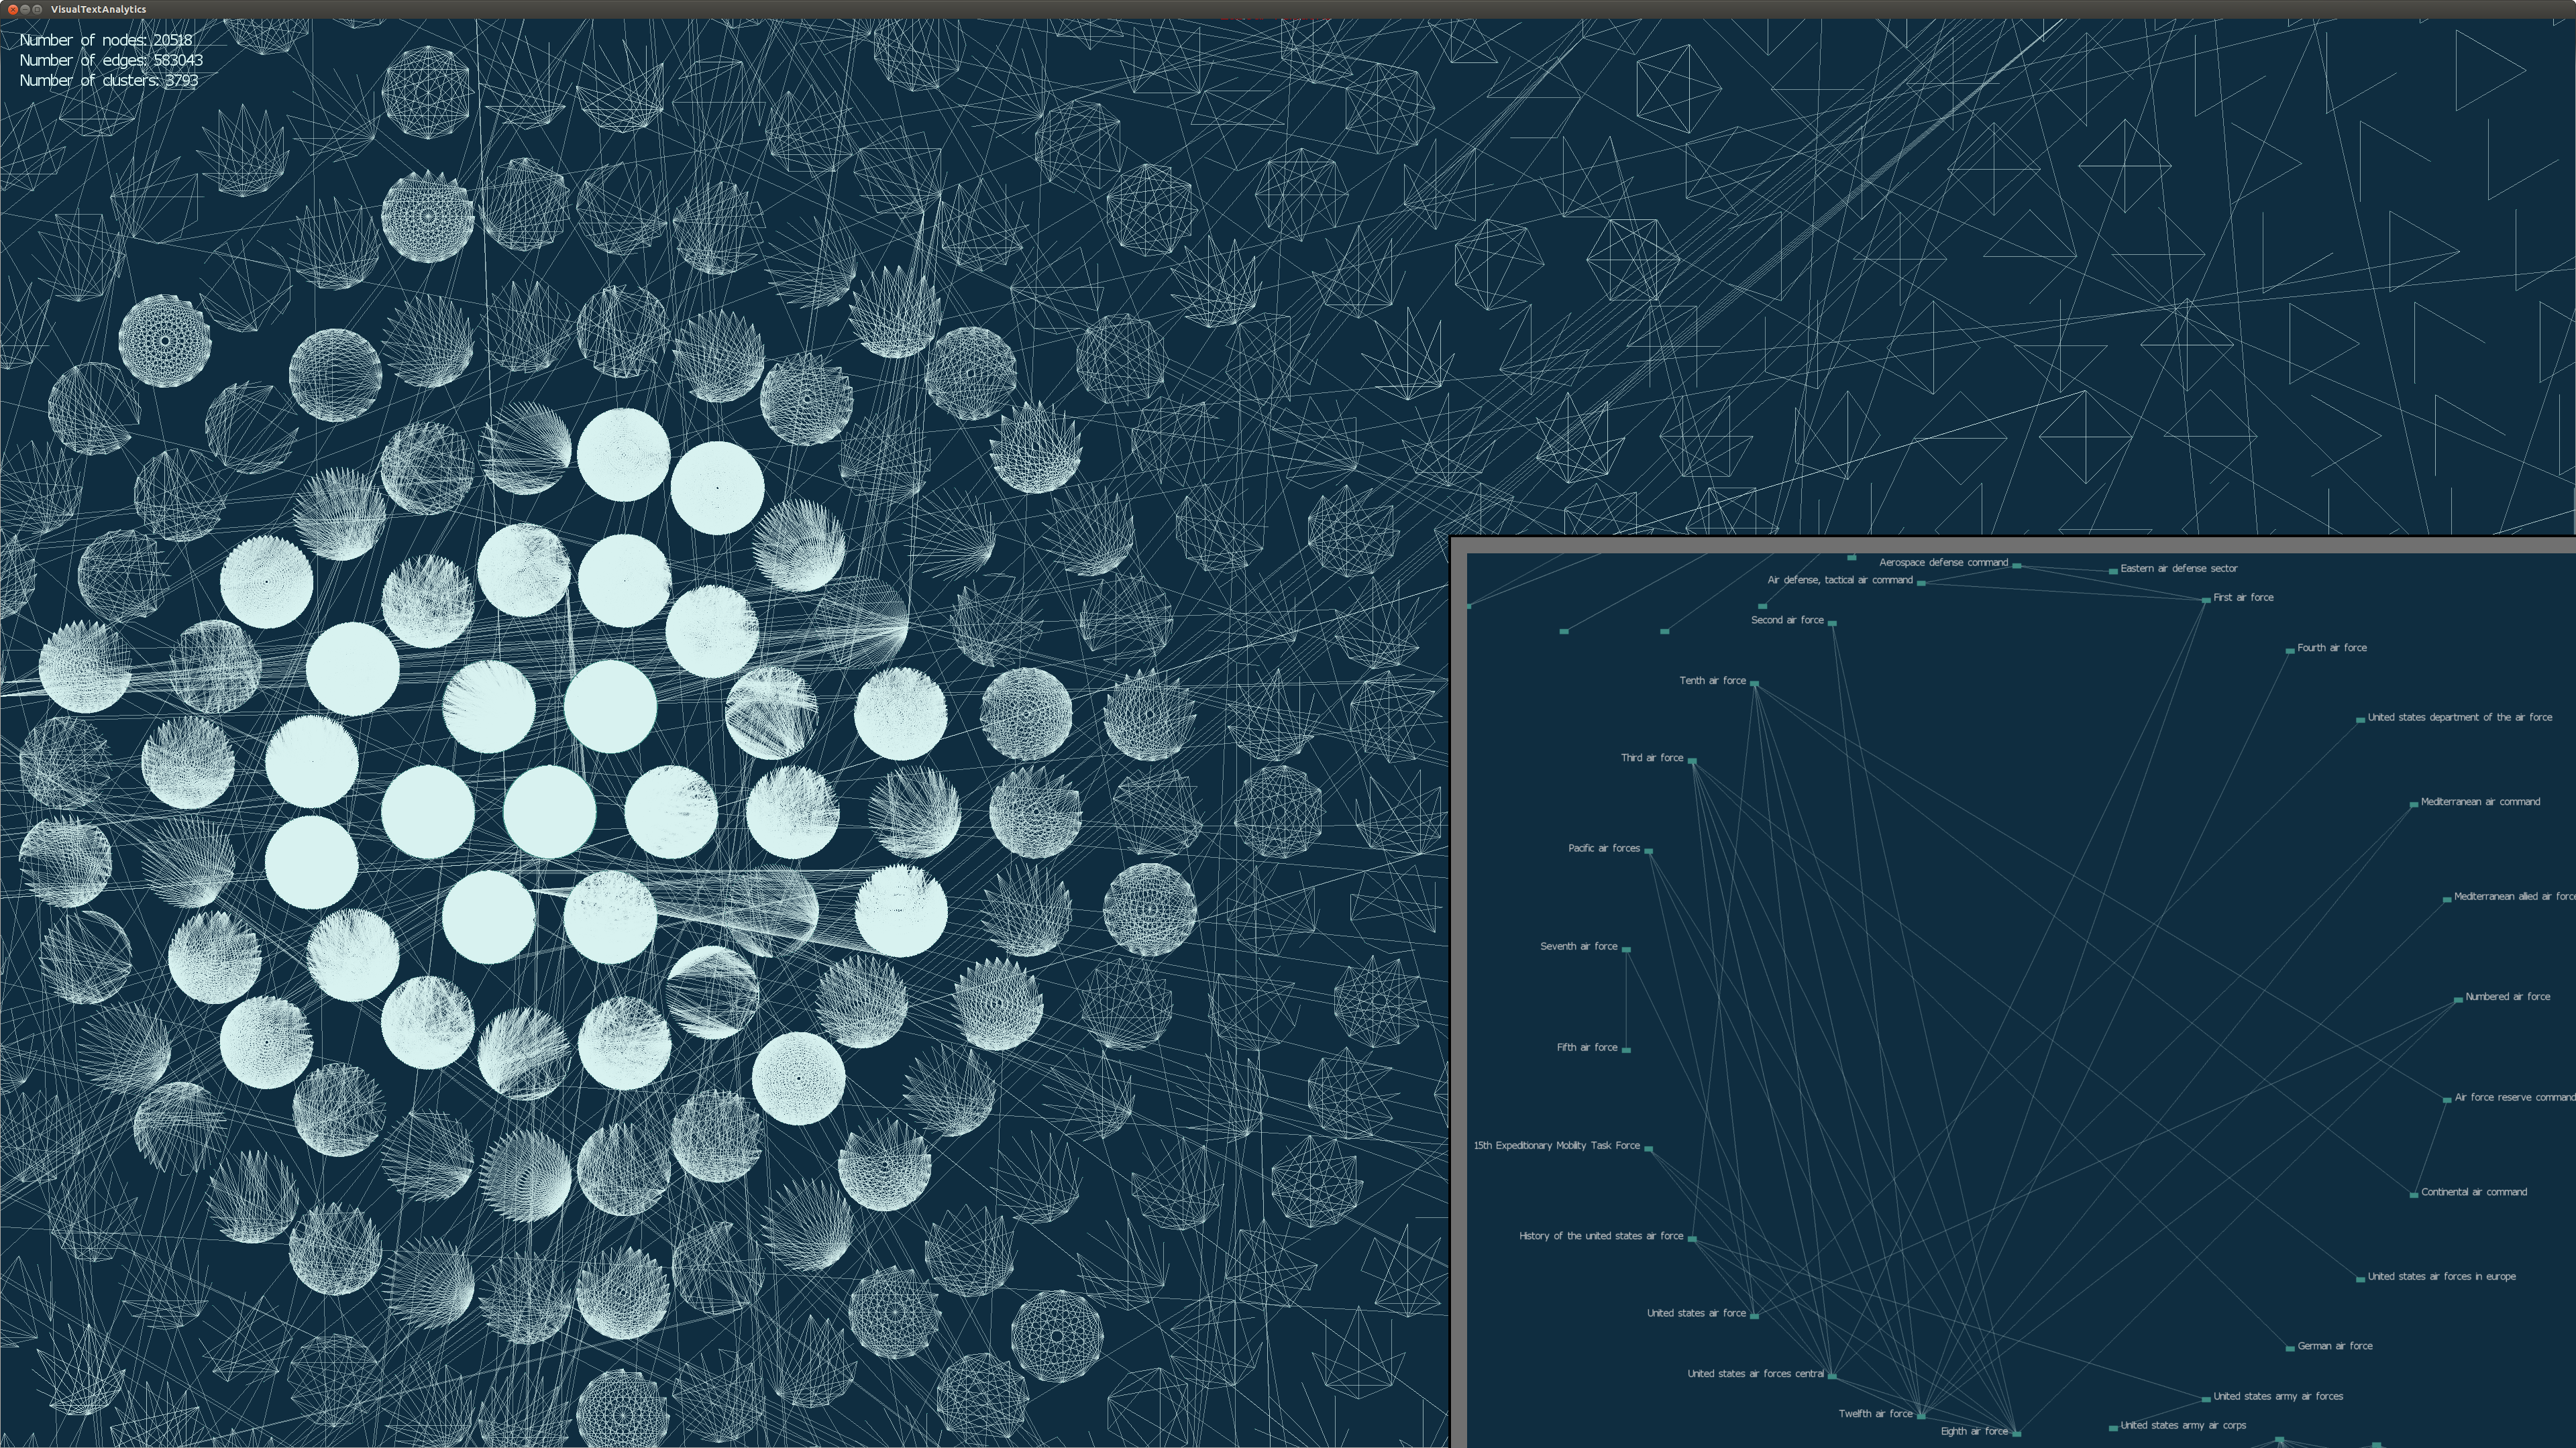
\includegraphics[width=\textwidth]{images/01_introduction/vta-cover.png}
\caption{Ausschnitt aus dem Projekt \textit{Visual Text Analytics}. Rechts unten ist ein Cluster im Fokus zu sehen. Der Hintergrund zeigt die Startvisualisierung mit einer Übersicht aller Cluster.}
\label{fig:vta-cover}
\end{figure}

\begin{figure}
    \centering
    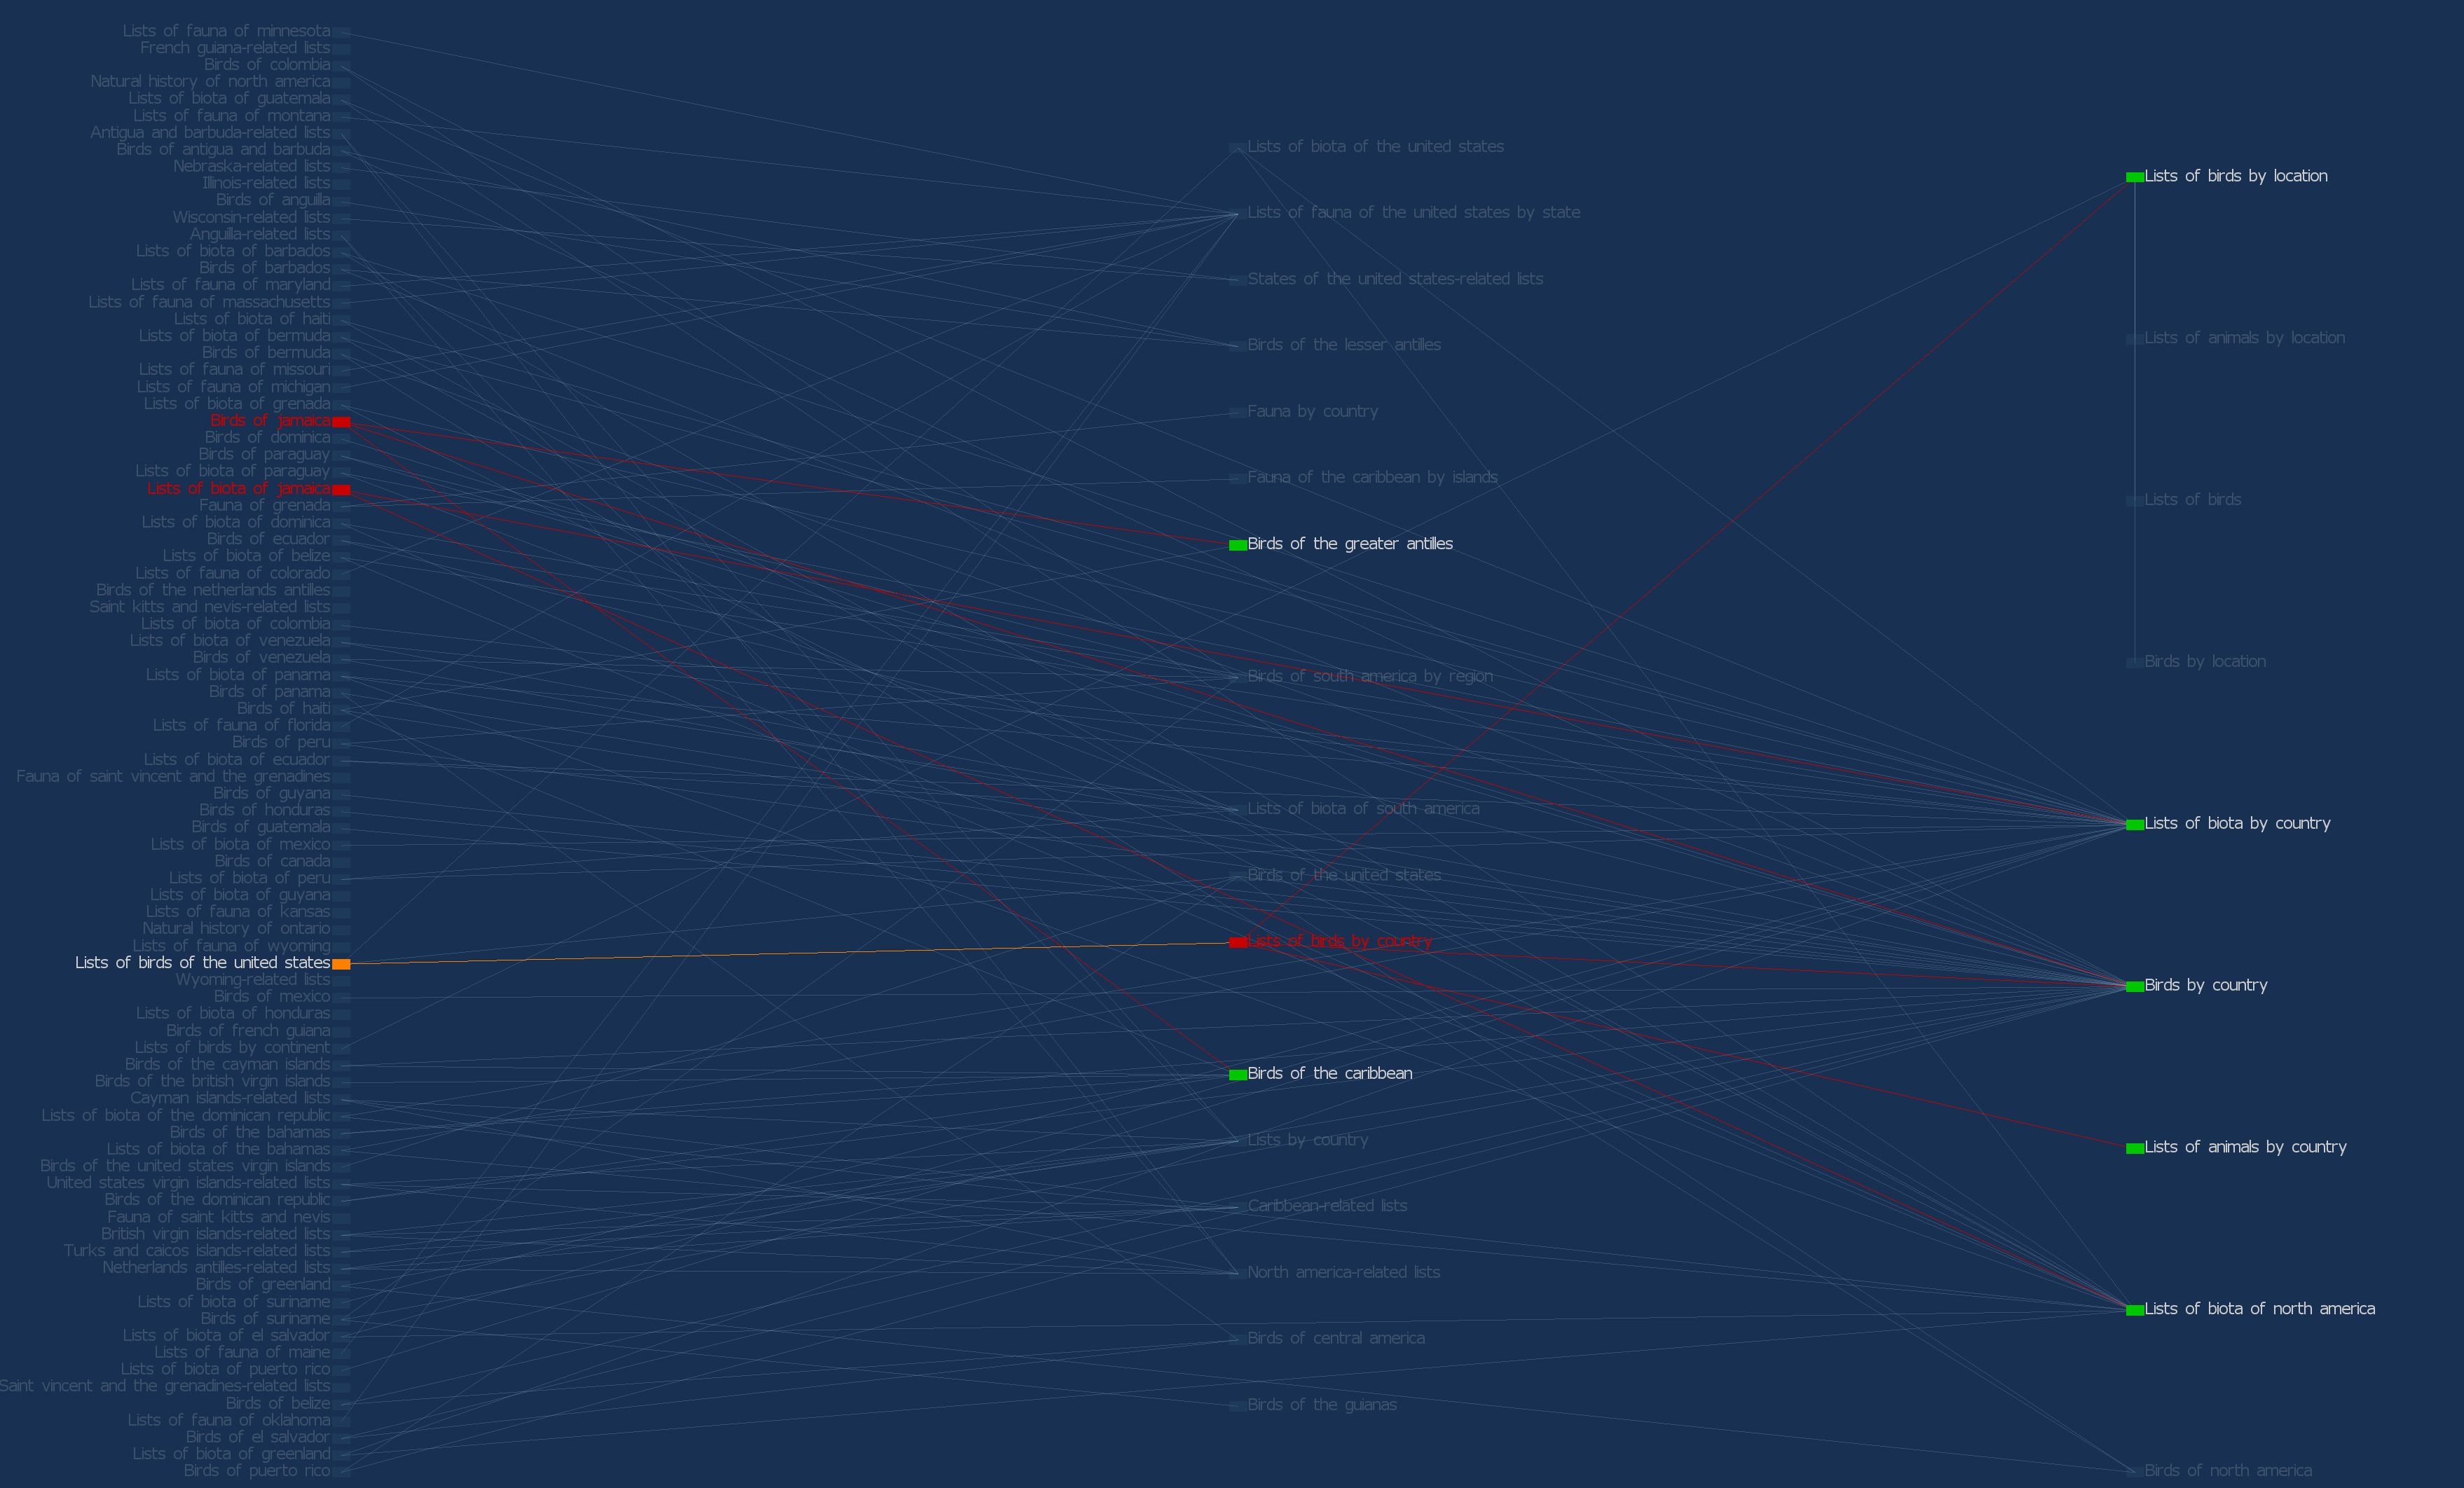
\includegraphics[width=\textwidth]{images/01_introduction/category-view.png}
    \caption{Ausschnitt des Kategoriengraphen. Die Knoten stellen Kategorien dar, die Kanten veranschaulichen die Verbindungen zwischen den Kategorien.\\ In diesem Bild wird die grün gefärbte Kategorie ausgewählt. Alle Knoten und Kanten ohne Verbindung zur ausgewählten Kategorie sind ausgegraut.}
    \label{fig:category-view}
\end{figure}
\todotext{Bild mit einer geclickten Kategorie}
















%NOTE
% Relevanz von Informationsvisualisierung\\
% Bezug auf das vorangegangene Projekt Visual Text Analytics\\
% einmal eine Abstrakte Motivation -> Darstellung Kategorienbaum + "Ahnlichkeiten
%
% Motivation aus dem vorg"anger Projekt -> konkreter Bezug auf fehlende Eigenschaften und Erkenntnisse
% defacto die einzige Visualisierung f"ur den Kategoriebaum der Wikipedia
% =========================================================

















% DRAFTS ============================
% Um die enorme Menge an Kanten, welche einen Vergleich zwischen zwei Artikeln repres"antiert, darstellen zu k"onnen, muss ein Schwellwert festgelegt werden, bevor die Visualisierng ausgef"uhrt wird.

% Ziel der Arbeit ist es, das Verst"andnis "uber die Kategoriestruktur und die "Ahnlichkeiten zwischen Artikeln der Wikipedia zu verbessern.
% F"ur die enorme Menge an Vergleichen zwischen Artikeln muss eine L"osung entwickelt werden, welche die Menge reduziert, somit f"ur den Computer darstellbar und f"ur den Menschen nachvollziehbar ist.
% Der Mittelpunkt der Arbeit ist die Darstellung der hierarchischen Struktur der Kategorien aus der Wikipedia.

% BULLET LIST ++++++++++++++++++++++++++++++++++++++++++++++++
% \begin{itemize}
%   \item Bedeutung des Wikipediadatensatzes
%   \item Kritikpunkte im Projekt Visual Text Analytics
%   \begin{itemize}
%     \item statisches Layout
%     \item fehlende M"oglichkeit zur Exploration der Daten
%     \item "Ubersicht der Visualisierung ist sehr undurchsichtig
%     \item Schwierigkeiten beim Nachvollziehen der Verbindungen zwischen den Artikeln untereinander
%     \item "Anderung des Schwellwertes f"ur "Ahnlichkeiten -> zu viele Kanten
%     \item fehlende M"oglichkeit, die Auswahl an Artikeln einzuschr"anken
%     \item Unterst"utzende Funktion zum Zusammenfassen von mehreren Artikeln -> Kategorien, Cluster
%     \item Artikelcluster mit vielen "Ahnlichkeiten zueinander sind schwer zu lesen
%     \item Kategorienbaum unzureichend als Unterzt"utzung neben den Artikeln
%   \end{itemize}
% \end{itemize}


% \begin{itemize}
%     \item Verbesserung des Verst"andnisses des "Ahnlichkeitsma"ses
%     \item Darstellung der Hierarchie von Kategorien
%     \begin{itemize}
%       \item Konstruktion eines Kategorienbaumes mit der M"oglichkeit der Exploration
%     \end{itemize}
%     \item Interaktive Visualisierung
%     \begin{itemize}
%       \item "Anderung des Schwellwerts zur Laufzeit
%     \end{itemize}
%     \item Exploration der Daten
%     \item Bezug zu anderen Datens"atzen: Autoren, Editierungen, etc.
% \end{itemize}














































% % ////////////////////////////////////
% \begin{figure}[H]
%     \centering
%     \begin{subfigure}[b]{0.96\textwidth}
%         \includegraphics[width=\textwidth]{images/01_introduction/motivation_temporal_superresolution_one.pdf}
%         \caption{3D video playback rate matching the low recording rate}
%         % \label{subfig:playback_rate_matching}
%     \end{subfigure}

% 	\vspace{1.0cm}

%     \begin{subfigure}[b]{0.96\textwidth}
%         \includegraphics[width=\textwidth]{images/01_introduction/motivation_temporal_superresolution_two.pdf}
%         \caption{3D video playback matching the video encoding standards to ensure persistence of fluid motion}
%         % \label{subfig:playback_rate_higher}
%     \end{subfigure}
%     \caption[Concept of Temporal Super Resolution in a 3D Video Player]{In this Figure, two different playback rates for a low frame rate recording of a 3D volume sequence is presented. The tick marks on the black arrows indicate the position of recorded frames. The blue arrows indicate the playback rate that matches the recording \subref{subfig:playback_rate_matching} and an increased playback rate \subref{subfig:playback_rate_higher} using temporal interpolation to provide the viewer with a impression of fluid motion. }
%     % \label{fig:temporal_superresolution}
% \end{figure}

%  \cite{VillanuevaEtAl:2016}